\documentclass[]{article}

\usepackage{amsmath}
\usepackage{amssymb}
\usepackage{graphicx}
\usepackage{subcaption}
\usepackage{hyperref}
\usepackage{algorithm}
\usepackage{algpseudocode}

\graphicspath{{../benchmark/plots/}{../benchmark/plots-FK/}}

\title{Benchmarking Quantum Computers via Verification Protocols}
\author{}
\date{}

\begin{document}

\maketitle

\section{Benchmarking}
\label{sec:benchmarking}

Verification protocols are most commonly discussed as tools for certifying a
single delegated computation. However, the information they produce --- in
particular, the failure rate of test rounds --- is meaningful beyond this
narrow use case. Under the sole assumption that the device behaves consistently
from round to round (i.i.d.\ across rounds), this failure rate is a stable
property of the device, independent of the specific computation being run.
Extracting and interpreting this information is therefore an additional
application of verification protocols, complementary to their primary role.

This observation was formalised by Frank et al.~\cite{frank2024}, who establish
a rigorous link between verification and benchmarking and show that any
verification protocol can be compiled into a certifiable benchmark for a class
of computations. In particular, they propose characterising quantum devices by
certifying 2D brickwork states of increasing dimensions $(N, D)$, yielding a
device profile of the form shown in their Figure~4. In the present work we
instantiate this approach concretely using the Veriphix verification framework:
we run the FK verification protocol on simulated circuits of varying dimensions,
and construct the resulting feasibility landscape explicitly as a function of
the round budget $R$ and security target $\varepsilon$. This benchmarking
application is one of two utilities of verification protocols demonstrated in
this paper, the other being noise estimation (Section~\ref{sec:hotgate}).

% TODO: Add simulation results for correlated depolarising and more complex
%       noise models to assess robustness of the benchmark beyond i.i.d. noise.

\subsection{From test rounds to a utility metric}
\label{subsec:utility}

When test rounds fail or pass, that carries information about the device's
noise. If the device behaves consistently throughout time (i.i.d.\ assumption),
this failure rate is stable: it does not depend on which specific computation
was run, nor on when the rounds were executed. Furthermore, since verification
is blind by construction, the failure rate is the same for \emph{all}
computations sharing the same brickwork dimensions $(N, D)$ --- the device
cannot distinguish between them.

The test-round failure rate therefore measures utility directly: it quantifies
how well the device handles any computation of dimension $(N, D)$, in the
worst case over all such computations. By asking whether the observed failure
rate is low enough to certify computation at dimension $(N, D)$ with security
$\varepsilon$ in $R$ rounds, one obtains a concrete, algorithm-independent
performance metric. This is the benchmark.

\subsection{Benchmarking protocol}
\label{subsec:bench-protocol}

\begin{algorithm}[H]
\caption{Verification-based feasibility benchmark}
\begin{algorithmic}[1]
\Require
  \begin{itemize}
    \item Set of circuit dimensions $\{(N_i, D_i)\}$ to probe
    \item Round budget $R$ (total number of rounds the experimenter can afford)
    \item Security target $\varepsilon$ (acceptable correctness error probability)
  \end{itemize}
\Ensure Feasibility landscape $\mathcal{F}$: the set of dimensions $(N, D)$ the device can safely run
\State $\mathcal{F} \leftarrow \emptyset$
\For{each circuit dimension $(N, D)$}
    \State Sample a collection of circuits of dimension $(N, D)$
    \State For each circuit, run the FK verification protocol with $T_{\mathrm{test}} = 100$ test rounds
    \State Let $f_k$ = number of failed test rounds for circuit $k$, out of $T_{\mathrm{test}}$
    \State Compute the average test-round failure rate across all circuits:
    \[
        \bar{p}(N, D) \;=\; \frac{1}{|\mathcal{C}|}\sum_{k \in \mathcal{C}} \frac{f_k}{T_{\mathrm{test}}}
    \]
    \State Query the verification machinery: what is the maximum tolerable noise rate $p^*(R, \varepsilon)$
           such that a device with failure rate $p^*$ can be certified within $R$ rounds at security $\varepsilon$?
    \If{$\bar{p}(N, D) \leq p^*(R, \varepsilon)$}
        \State Label dimension $(N, D)$ as \emph{safe}: add it to $\mathcal{F}$
    \EndIf
\EndFor
\State \Return $\mathcal{F}$
\end{algorithmic}
\end{algorithm}

The key step is the comparison $\bar{p}(N,D) \leq p^*(R, \varepsilon)$: the observed failure
rate is tested against the maximum noise the protocol can certify, given the available round
budget $R$ and the desired security $\varepsilon$. The output $\mathcal{F}$ is the feasibility
landscape of the device under its observed noise.

\subsection{The verification protocol}
\label{subsec:protocol}

% TODO: brief self-contained description of the protocol mechanics
%   (client prepares single-qubit states, server performs MBQC on brickwork
%    state of dimensions N x D, traps allow client to detect errors;
%    reference FK / UBQC as appropriate)

\subsection{Main result (informal)}
\label{subsec:result}

Informally, the main result is the following. Fix a threshold $w/t$ --- the
maximum admissible fraction of test-round failures --- and run the verification
protocol on a brickwork state of dimensions $(N, D)$. If the observed failure
rate stays below this threshold, then the output of the computation is, with
probability at least $1 - \varepsilon$, indistinguishable from the ideal
output. Conversely, if the noise rate exceeds the threshold, the protocol
rejects with overwhelming probability, protecting the Client from acting on a
corrupted result.

More precisely, one proves that the protocol with threshold $w/t$ is
$\varepsilon$-close to the ideal resource, provided the circuit-level noise
rate $p$ satisfies $p < w/t - \delta$, where the security gap $\delta$
controls the exponential decay of $\varepsilon$ with the number of test rounds.
The number of rounds $R$ required to achieve a given $(\varepsilon, \delta)$
pair constitutes the round overhead of the benchmark.

\subsection{Feasibility landscape}
\label{subsec:landscape}

The round overhead can be turned into a concrete benchmarking criterion. For
given circuit dimensions $(N, D)$ and a given security target $\varepsilon$,
the verification machinery determines the minimum number of rounds $R$ required
to certify the computation. We then ask: is this $R$ feasible in practice?
Varying both $\varepsilon$ and the allowed budget $R$ produces a
two-dimensional feasibility landscape: the set of $(R, \varepsilon)$ pairs for
which a circuit of dimensions $(N, D)$ can be certified.

Aggregating this landscape over circuit dimensions gives a heatmap in which
each cell indicates the maximum certifiable $(N, D)$ for a given
$(R, \varepsilon)$ pair. Since the circuit dimension is two-dimensional, we
reduce to a scalar size via the brick count $B(N, D)$ (defined in
Eq.~\eqref{eq:bricks}) for display purposes, while the axes of the heatmap
remain $R$ and $\varepsilon$. The heatmap directly answers the question: given
a round budget and a security target, how large a computation can this device
run?

\subsection{Simulation}
\label{subsec:simulation}

Circuits are parameterised by the number of qubits $N$ and the depth $D$, and
are generated randomly with a BQP error rate of $0.1$, yielding 100 circuits
per $(N, D)$ dimension. Each circuit is transpiled onto a pattern over a
brickwork state of dimensions $N \times D$, whose entangling structure
determines the circuit size.

The brickwork transpilation alternates between two layer parities: even-indexed
layers contain $\lfloor N/2 \rfloor$ bricks, and odd-indexed layers contain
$\lfloor (N-1)/2 \rfloor$ bricks. Over $D$ layers --- $\lceil D/2 \rceil$ even
and $\lfloor D/2 \rfloor$ odd --- the total brick count is
\begin{equation}
  B(N,D) = \left\lceil \frac{D}{2} \right\rceil \left\lfloor \frac{N}{2} \right\rfloor
          + \left\lfloor \frac{D}{2} \right\rfloor \left\lfloor \frac{N-1}{2} \right\rfloor.
  \label{eq:bricks}
\end{equation}
For odd $N$ this simplifies to $B = D(N-1)/2$, since both layer types
contribute $(N-1)/2$ bricks per layer. For even $N$ it becomes $B = DN/2 -
\lfloor D/2 \rfloor$. As a concrete example, for $N = 7$ and $D = 8$ (odd
$N$), $B = 8 \times 3 = 24$ bricks.

Verification was performed using Veriphix under a depolarising noise model
applied to entangling gates, at fixed noise probability $p$. Two representative
noise regimes were studied: $p = 6 \times 10^{-4}$ and $p = 2 \times 10^{-3}$.
For each circuit, 100 test rounds were drawn using Random Traps (detection rate
$1/2$) and the resulting feasibility landscape was computed. The simulation was
then repeated independently using the FK trap construction in place of Random
Traps, enabling a direct comparison of the two trap designs at identical noise
levels.

\begin{figure}[t]
  \centering
  \begin{subfigure}[b]{0.48\columnwidth}
    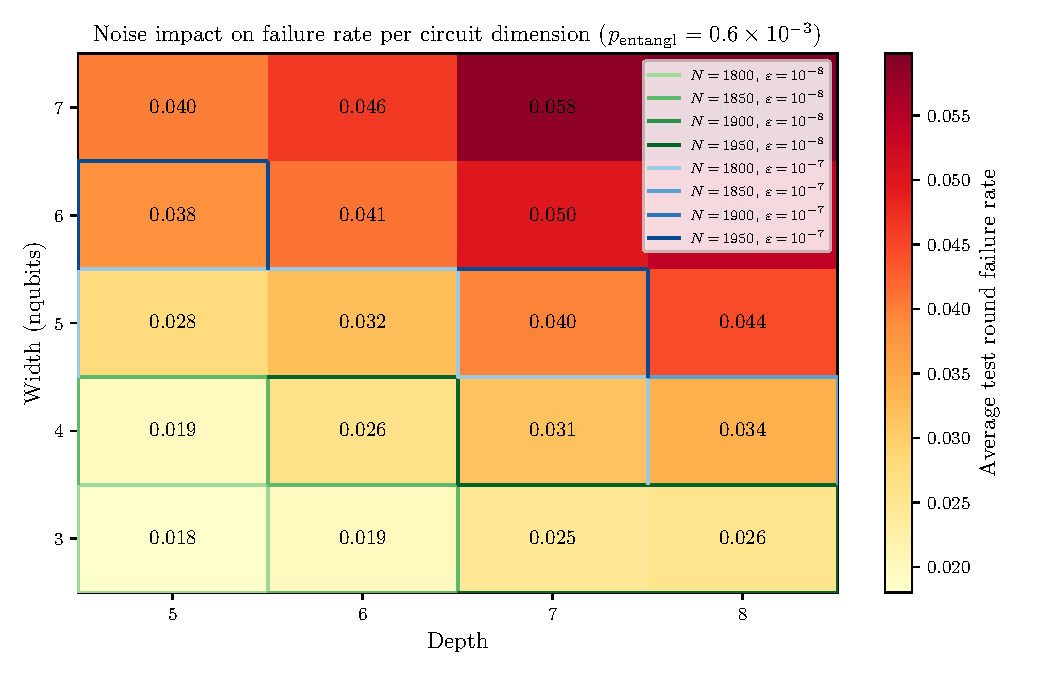
\includegraphics[width=\textwidth]{discrete_p6e-04_bqp0.1.pdf}
    \caption{$p = 6\times10^{-4}$.}
  \end{subfigure}
  \hfill
  \begin{subfigure}[b]{0.48\columnwidth}
    
\includegraphics[width=\textwidth]{discrete_p2e-03_bqp0.1.pdf}
    \caption{$p = 2\times10^{-3}$.}
  \end{subfigure}
  \caption{%
    Discrete feasibility plot for Random Trap verification at two noise levels.
    Each point represents a circuit dimension $(N, D)$; filled markers indicate
    dimensions certified as feasible (test-round failure rate below threshold),
    open markers indicate infeasible dimensions. The frontier (dashed) marks
    the boundary of certified feasibility as a function of the round budget $R$
    and target security $\varepsilon$.
  }
  \label{fig:discrete_rt}
\end{figure}

\begin{figure}[t]
  \centering
  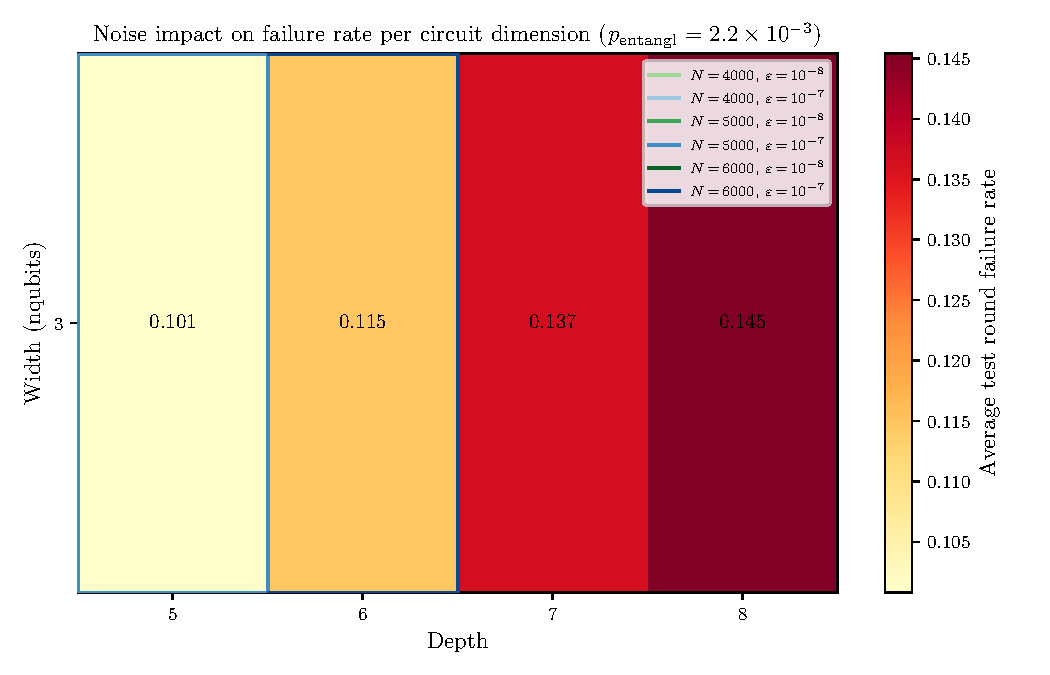
\includegraphics[width=0.6\columnwidth]{../benchmark/plots-FK/discrete_p2e-03_bqp0.1.pdf}
  \caption{%
    Discrete feasibility plot for FK verification at $p = 2\times10^{-3}$.
    Layout follows Fig.~\ref{fig:discrete_rt}. Comparison with
    Fig.~\ref{fig:discrete_rt}(b) isolates the effect of the trap construction
    on the certified feasibility frontier.
  }
  \label{fig:discrete_fk}
\end{figure}

\begin{figure}[t]
  \centering
  \begin{subfigure}[b]{0.48\columnwidth}
    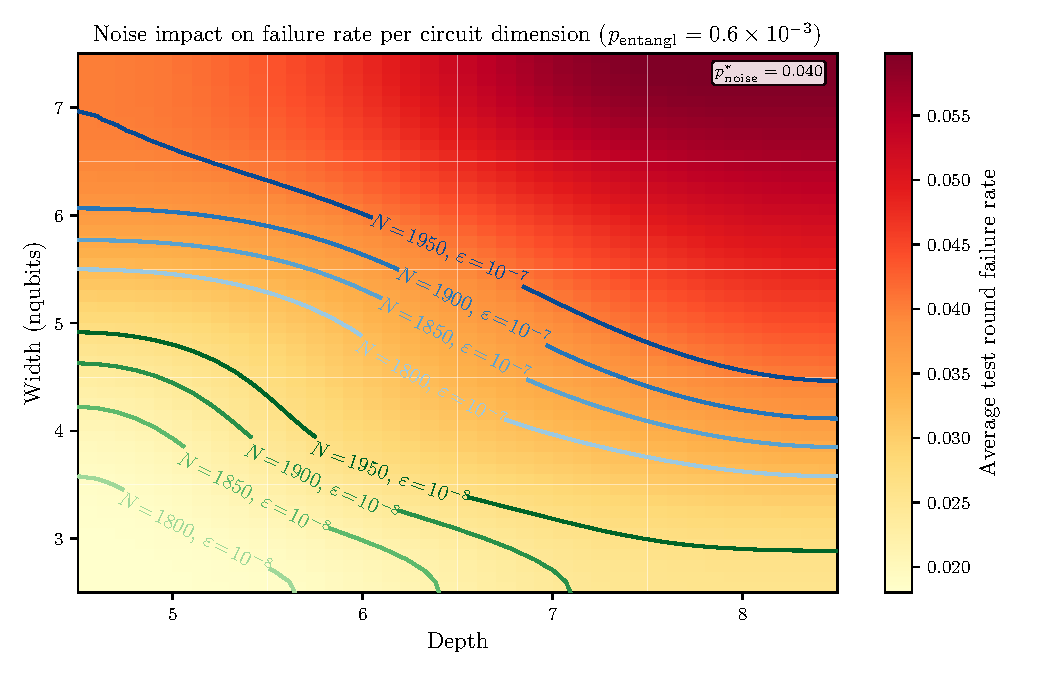
\includegraphics[width=\textwidth]{heatmap_p6e-04_bqp0.1.pdf}
    \caption{$p = 6\times10^{-4}$.}
  \end{subfigure}
  \hfill
  \begin{subfigure}[b]{0.48\columnwidth}
    
\includegraphics[width=\textwidth]{heatmap_p2e-03_bqp0.1.pdf}
    \caption{$p = 2\times10^{-3}$.}
  \end{subfigure}
  \caption{%
    Feasibility heatmaps (Random Traps) at two noise levels. Colour encodes the
    maximum brick count $B(N, D)$ certifiable as feasible, as a function of the
    total round budget $R$ (horizontal axis) and security target $\varepsilon$
    (vertical axis). The discrete feasibility data are interpolated via bicubic
    smoothing. Darker regions correspond to larger certifiable circuit sizes;
    white regions indicate that no circuit dimension $(N, D)$ can be certified
    under the given $(R, \varepsilon)$ pair.
  }
  \label{fig:heatmap_rt}
\end{figure}

\begin{figure}[t]
  \centering
  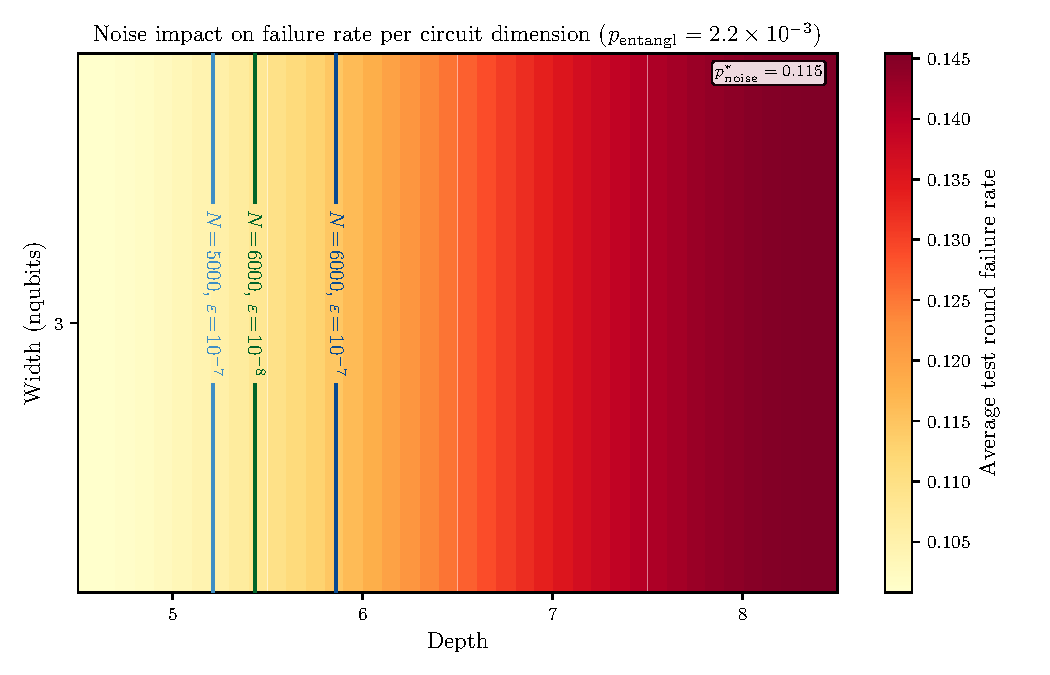
\includegraphics[width=0.6\columnwidth]{../benchmark/plots-FK/heatmap_p2e-03_bqp0.1.pdf}
  \caption{%
    Feasibility heatmap for FK verification at $p = 2\times10^{-3}$.
    Layout follows Fig.~\ref{fig:heatmap_rt}. Direct comparison with
    Fig.~\ref{fig:heatmap_rt}(b) quantifies the impact of the trap construction
    on the certifiable feasibility landscape.
  }
  \label{fig:heatmap_fk}
\end{figure}

\end{document}
